\documentclass[11pt]{article}

\usepackage{fullpage}
\usepackage{newtxtext}
\usepackage[T1]{fontenc}
\usepackage{hyperref,microtype,pdfsync}
\usepackage{amsmath,amsfonts,amssymb,amsthm}
\usepackage{mathtools}
\usepackage{fancyhdr}
\usepackage{graphicx}
\usepackage{algorithm,algorithmic}

%%% BLACKBOARD SYMBOLS

% hyperref package defines C and G, undefined to avoid conflicts
\let\C\relax
\let\G\relax
\newcommand{\C}{\ensuremath{\mathbb{C}}}
\newcommand{\D}{\ensuremath{\mathbb{D}}}
\newcommand{\F}{\ensuremath{\mathbb{F}}}
\newcommand{\G}{\ensuremath{\mathbb{G}}}
\newcommand{\J}{\ensuremath{\mathbb{J}}}
\newcommand{\N}{\ensuremath{\mathbb{N}}}
\newcommand{\Q}{\ensuremath{\mathbb{Q}}}
\newcommand{\R}{\ensuremath{\mathbb{R}}}
\newcommand{\T}{\ensuremath{\mathbb{T}}}
\newcommand{\Z}{\ensuremath{\mathbb{Z}}}
\newcommand{\QR}{\ensuremath{\mathbb{QR}}}

\newcommand{\Zt}{\ensuremath{\Z_t}}
\newcommand{\Zp}{\ensuremath{\Z_p}}
\newcommand{\Zq}{\ensuremath{\Z_q}}
\newcommand{\ZN}{\ensuremath{\Z_N}}
\newcommand{\Zps}{\ensuremath{\Z_p^*}}
\newcommand{\ZNs}{\ensuremath{\Z_N^*}}
\newcommand{\JN}{\ensuremath{\J_N}}
\newcommand{\QRN}{\ensuremath{\QR_{N}}}
\newcommand{\QRp}{\ensuremath{\QR_{p}}}

%%% THEOREM COMMANDS

\theoremstyle{plain}            % following are "theorem" style
\newtheorem{theorem}{Theorem}[section]
\newtheorem{lemma}[theorem]{Lemma}
\newtheorem{corollary}[theorem]{Corollary}
\newtheorem{proposition}[theorem]{Proposition}
\newtheorem{claim}[theorem]{Claim}
\newtheorem{fact}[theorem]{Fact}

\theoremstyle{definition}       % following are def style
\newtheorem{definition}[theorem]{Definition}
\newtheorem{conjecture}[theorem]{Conjecture}
\newtheorem{example}[theorem]{Example}
\newtheorem{protocol}[theorem]{Protocol}

\theoremstyle{remark}           % following are remark style
\newtheorem{remark}[theorem]{Remark}
\newtheorem{note}[theorem]{Note}
\newtheorem{exercise}[theorem]{Exercise}

% equation numbering style
\numberwithin{equation}{section}

%%% GENERAL COMPUTING

\newcommand{\bit}{\ensuremath{\set{0,1}}}
\newcommand{\pmone}{\ensuremath{\set{-1,1}}}

% asymptotics
\DeclareMathOperator{\poly}{poly}
\DeclareMathOperator{\polylog}{polylog}
\DeclareMathOperator{\negl}{negl}
\newcommand{\Otil}{\ensuremath{\tilde{O}}}

% probability/distribution stuff
\DeclareMathOperator*{\E}{E}
\DeclareMathOperator*{\Var}{Var}

% sets in calligraphic type
\newcommand{\calD}{\ensuremath{\mathcal{D}}}
\newcommand{\calF}{\ensuremath{\mathcal{F}}}
\newcommand{\calG}{\ensuremath{\mathcal{G}}}
\newcommand{\calH}{\ensuremath{\mathcal{H}}}
\newcommand{\calX}{\ensuremath{\mathcal{X}}}
\newcommand{\calY}{\ensuremath{\mathcal{Y}}}

% types of indistinguishability
\newcommand{\compind}{\ensuremath{\stackrel{c}{\approx}}}
\newcommand{\statind}{\ensuremath{\stackrel{s}{\approx}}}
\newcommand{\perfind}{\ensuremath{\equiv}}

% font for general-purpose algorithms
\newcommand{\algo}[1]{\ensuremath{\mathsf{#1}}}
% font for general-purpose computational problems
\newcommand{\problem}[1]{\ensuremath{\mathsf{#1}}}
% font for complexity classes
\newcommand{\class}[1]{\ensuremath{\mathsf{#1}}}

% complexity classes and languages
\renewcommand{\P}{\class{P}}
\newcommand{\BPP}{\class{BPP}}
\newcommand{\NP}{\class{NP}}
\newcommand{\coNP}{\class{coNP}}
\newcommand{\AM}{\class{AM}}
\newcommand{\coAM}{\class{coAM}}
\newcommand{\IP}{\class{IP}}

%%% "LEFT-RIGHT" PAIRS OF SYMBOLS

%% NOTE: this requires \usepackage{mathtools} in the document preamble

% inner product
\DeclarePairedDelimiter\inner{\langle}{\rangle}
% absolute value
\DeclarePairedDelimiter\abs{\lvert}{\rvert}
% a set
\DeclarePairedDelimiter\set{\{}{\}}
% parens
\DeclarePairedDelimiter\parens{(}{)}
% tuple, alias for parens
\DeclarePairedDelimiter\tuple{(}{)}
% square brackets
\DeclarePairedDelimiter\bracks{[}{]}
% rounding off
\DeclarePairedDelimiter\round{\lfloor}{\rceil}
% floor function
\DeclarePairedDelimiter\floor{\lfloor}{\rfloor}
% ceiling function
\DeclarePairedDelimiter\ceil{\lceil}{\rceil}
% length of some vector, element
\DeclarePairedDelimiter\length{\lVert}{\rVert}
% "lifting" of a residue class
\DeclarePairedDelimiter\lift{\llbracket}{\rrbracket}
\DeclarePairedDelimiter\len{\lvert}{\rvert}

%%% CRYPTO-RELATED NOTATION

% KEYS AND RELATED

\newcommand{\key}[1]{\ensuremath{#1}}

\newcommand{\pk}{\key{pk}}
\newcommand{\vk}{\key{vk}}
\newcommand{\sk}{\key{sk}}
\newcommand{\mpk}{\key{mpk}}
\newcommand{\msk}{\key{msk}}
\newcommand{\fk}{\key{fk}}
\newcommand{\id}{id}
\newcommand{\keyspace}{\ensuremath{\mathcal{K}}}
\newcommand{\msgspace}{\ensuremath{\mathcal{M}}}
\newcommand{\ctspace}{\ensuremath{\mathcal{C}}}
\newcommand{\tagspace}{\ensuremath{\mathcal{T}}}
\newcommand{\idspace}{\ensuremath{\mathcal{ID}}}

\newcommand{\concat}{\ensuremath{\|}}

% GAMES

% advantage
\newcommand{\advan}{\ensuremath{\mathbf{Adv}}}

% different attack models
\newcommand{\attack}[1]{\ensuremath{\text{#1}}}

\newcommand{\atk}{\attack{atk}} % dummy attack
\newcommand{\indcpa}{\attack{ind-cpa}}
\newcommand{\indcca}{\attack{ind-cca}}
\newcommand{\anocpa}{\attack{ano-cpa}} % anonymous
\newcommand{\anocca}{\attack{ano-cca}}
\newcommand{\euacma}{\attack{eu-acma}} % forgery: adaptive chosen-message
\newcommand{\euscma}{\attack{eu-scma}} % forgery: static chosen-message
\newcommand{\suacma}{\attack{su-acma}} % strongly unforgeable

% ADVERSARIES
\newcommand{\attacker}[1]{\ensuremath{\mathcal{#1}}}

\newcommand{\Adv}{\attacker{A}}
\newcommand{\AdvA}{\attacker{A}}
\newcommand{\AdvB}{\attacker{B}}
\newcommand{\Dist}{\attacker{D}}
\newcommand{\Sim}{\attacker{S}}
\newcommand{\Ora}{\attacker{O}}
\newcommand{\Inv}{\attacker{I}}
\newcommand{\For}{\attacker{F}}

% CRYPTO SCHEMES

\newcommand{\scheme}[1]{\ensuremath{\text{#1}}}

% pseudorandom stuff
\newcommand{\prg}{\algo{PRG}}
\newcommand{\prf}{\algo{PRF}}
\newcommand{\prp}{\algo{PRP}}

% symmetric-key cryptosystem
\newcommand{\skc}{\scheme{SKC}}
\newcommand{\skcgen}{\algo{Gen}}
\newcommand{\skcenc}{\algo{Enc}}
\newcommand{\skcdec}{\algo{Dec}}

% public-key cryptosystem
\newcommand{\pkc}{\scheme{PKC}}
\newcommand{\pkcgen}{\algo{Gen}}
\newcommand{\pkcenc}{\algo{Enc}} % can also use \kemenc and \kemdec
\newcommand{\pkcdec}{\algo{Dec}}

% digital signatures
\newcommand{\sig}{\scheme{SIG}}
\newcommand{\siggen}{\algo{Gen}}
\newcommand{\sigsign}{\algo{Sign}}
\newcommand{\sigver}{\algo{Ver}}

% message authentication code
\newcommand{\mac}{\scheme{MAC}}
\newcommand{\macgen}{\algo{Gen}}
\newcommand{\mactag}{\algo{Tag}}
\newcommand{\macver}{\algo{Ver}}

% key-encapsulation mechanism
\newcommand{\kem}{\scheme{KEM}}
\newcommand{\kemgen}{\algo{Gen}}
\newcommand{\kemenc}{\algo{Encaps}}
\newcommand{\kemdec}{\algo{Decaps}}

% identity-based encryption
\newcommand{\ibe}{\scheme{IBE}}
\newcommand{\ibesetup}{\algo{Setup}}
\newcommand{\ibeext}{\algo{Ext}}
\newcommand{\ibeenc}{\algo{Enc}}
\newcommand{\ibedec}{\algo{Dec}}

% hierarchical IBE (as key encapsulation)
\newcommand{\hibe}{\scheme{HIBE}}
\newcommand{\hibesetup}{\algo{Setup}}
\newcommand{\hibeext}{\algo{Extract}}
\newcommand{\hibeenc}{\algo{Encaps}}
\newcommand{\hibedec}{\algo{Decaps}}

% binary tree encryption (as key encapsulation)
\newcommand{\bte}{\scheme{BTE}}
\newcommand{\btesetup}{\algo{Setup}}
\newcommand{\bteext}{\algo{Extract}}
\newcommand{\bteenc}{\algo{Encaps}}
\newcommand{\btedec}{\algo{Decaps}}

% trapdoor functions
\newcommand{\tdf}{\scheme{TDF}}
\newcommand{\tdfgen}{\algo{Gen}}
\newcommand{\tdfeval}{\algo{Eval}}
\newcommand{\tdfinv}{\algo{Invert}}
\newcommand{\tdfver}{\algo{Ver}}

%%% PROTOCOLS

\newcommand{\out}{\text{out}}
\newcommand{\view}{\text{view}}

%%% COMMANDS FOR LECTURES/HOMEWORKS

\newcommand{\lecheader}{%
  \chead{\large \textbf{Lecture \lecturenum\\\lecturetopic}}

  \lhead{\small \textbf{Theory of Cryptography}\\}

  \rhead{\small \textbf{Instructor:
      \href{http://www.eecs.umich.edu/~cpeikert/}{Chris Peikert}\\Scribe:
      \scribename}}

  \setlength{\headheight}{20pt}
  \setlength{\headsep}{16pt}
}


% VARIABLES

\newcommand{\lecturenum}{8}
\newcommand{\lecturetopic}{Pseudorandom Functions}
\newcommand{\scribename}{Indranil Banerjee}

% END OF VARIABLES

\lecheader

\pagestyle{plain}               % default: no special header

\begin{document}

\thispagestyle{fancy}           % first page should have special header

% LECTURE MATERIAL STARTS HERE

\section{Recap: Pseudorandom Generators}
\label{sec:recap:-pseud-gener}

\begin{enumerate}
\item It is possible to construct a hard-core predicate for any
  one-way function.  Let $f: \{0,1\}^{*} \rightarrow \{0,1\}^{*}$ be
  any one-way function (or permutation).  We define $f'(r,x) =
  (r,f(x))$ for $\len{r} = \len{x}$.  Then $f'$ is also a one way
  function (or permutation, respectively), and $h(r,x) = \inner{r,x}
  \bmod 2$ is a hard core predicate for $f'$.
\item A pseudorandom generator exists under the assumption that a
  one-way permutation exists.  Formally, if $f$ is a OWP and $h$ is a
  hard-core predicate for $f$, then $G(s) = (f(s), h(s))$ is a PRG
  with output length $\ell(n) = n+1$.
\item If there exists a PRG $G(s) = (f(s), h(s))$ with output length
  $\ell(n) = n+1$, then
  \[G'(s) = (h(s), h(f(s)), h(f^{(2)}(s)), \cdots ,h(f^{(m-1)}(s))) \]
  is a PRG of output length $m$ for any $m = \poly(\abs{s})$.
\end{enumerate}

While it is well-known that the existence of a PRG implies that a OWF
must exist, is the converse also true?  That is, does the existence of
a one-way function also imply that a pseudorandom generator must
exist?  In fact, this turns out to be true as well.  Hastad,
Impagliazzo, Levin, and Luby established in $1989$ that a PRG can be
constructed from any OWF.  Their construction is much more complicated
than the one for OWPs, because it must address the issue that the OWF
$f$ may be very ``unstructured,'' and thus the distribution of $f(x)$
may be very different from uniform, even when $x$ is uniform.  The
HILL PRG construction utilizes a random seed of length $n^{10}$ for a
OWF of input length $n$.  The details of the construction are beyond
the scope of this class.

\section{Pseudorandom Functions}
\label{sec:pseud-funct}

\subsection{Preliminary Concepts}
\label{sec:preliminary-concepts}

Having already developed a precise definition for a pseudorandom
\emph{string} of bits, a natural extension is, what would a random
\emph{function} look like?

A function from $\bit^{n}$ to $\bit$ is given by specifying an output
bit for every one of its inputs, of which there are $2^{n}$.
Therefore, the set of \emph{all} functions from $\bit^{n}$ to $\bit$
contains exactly $2^{2^{n}}$ functions; a ``random function'' (with
this domain and range) is a uniformly choice from this set.  Such a
function can also be viewed as a uniformly random $2^{n}$-bit string,
which simply lists all the function's outputs.  However, stated this
way, it is impossible to even look at the entire string efficiently
(in $\poly(n)$ time).  Therefore, we define a model in which we give
\emph{oracle} access to a function.

Writing $\Adv^{f}$ signifies that $\Adv$ has query access to $f$,
i.e., $\Adv$ can (adaptively) query the oracle on any input $x$ and
receive the output $f(x)$.  However, $\Adv$ only has a
``\emph{black-box}'' (input/output) view of $f$, without any knowledge
of how the function $f$ is evaluated.

\begin{definition}[Oracle indistinguishability]
  Let $\Ora = \{O_{n}\}$ and $\Ora'=\{O'_{n}\}$ be ensembles of
  probability distributions over functions from
  $\bit^{\ell_{1}(n)}$ to $\bit^{\ell_{2}(n)}$, for some
  $\ell_{1}(n), \ell_{2}(n) = \poly(n)$.  We say that $\Ora \compind
  \Ora'$ if, for all nuppt distinguishers $\Dist$,
  \[\advan_{\Ora,\Ora'}(\Dist) :=
  \abs*{\Pr_{f \gets O_{n}}[\Dist^{f}(1^n) = 1] - \Pr_{f \gets
      O'_{n}}[\Dist^{f}(1^n) = 1]} = \negl(n). \]
\end{definition}

Naturally, we say that $\Ora = \{O_{n}\}$ is \emph{pseudorandom} if \[
\Ora \compind \set*{U\parens*{\bit^{\ell_{1}(n)} \to
    \bit^{\ell_{2}(n)}}}, \] i.e., if no efficient adversary can
distinguish (given only oracle access) between a function sampled
according to $O_n$, and a uniformly random function, with more than
negligible advantage.

\begin{definition}[PRF Family]
  A family $\set*{f_{s}: \bit^{\ell_{1}(n)} \rightarrow
    \bit^{\ell_2(n)}}_{s \in \bit^{n}}$ is a \emph{pseudorandom
    function family} if it is:
  \begin{itemize}
  \item \emph{Efficiently computable}: there exists a deterministic
    polynomial-time algorithm $F$ such that $F(s,x) = f_{s}(x)$ for
    all $s \in \bit^{n}$ and $x \in \bit^{\ell_{1}(n)}$.
  \item \emph{Pseudorandom}: $\set*{U(\set{f_{s}})}$ is
    pseudorandom.
  \end{itemize}
\end{definition}

Having developed a precise definition of a pseudorandom family of
functions, the natural questions arises: Does such a primitive even
exist?  And under what assumptions?

Notice that if $\ell_{1}(n) = O(\log n)$, all the outputs values of a
function $f : \bit^{\ell_{1}(n)} \to \bit^{\ell_{2}(n)}$ can be
written down as a string of exactly $2^{\ell_{1}(n)} \cdot \ell_{2}(n)
= \poly(n)$ bits.  Moreover, all the function values can be queried in
polynomial time, given oracle access.  Therefore, a PRF family with
$O(\log n)$-length input may be seen as a PRG, and vice-versa.  But do
there exist PRF families with longer input lengths --- say, $n$?

\subsection{Constructing PRFs}
\label{sec:constructing-prfs}

\begin{theorem}
  \label{thm:prg-implies-prf}
  If a pseudorandom generator exists (i.e., if a one-way function
  exists), then a pseudorandom function family exists for any
  $\ell_{1}(n), \ell_{2}(n) = \poly(n)$.
\end{theorem}

At first glance, this theorem may seem completely absurd.  The number
of functions in the family $\set{f_{s}}$ with a seed length $\len{s} =
n$ is at most $2^n$, whereas the total number of functions overall
(even with just one-bit outputs) is at least $2^{2^{n}}$.  Therefore,
our function family is $\approx 2^{-2^{n}}$-sparse, i.e., the family
$\set{f_s}$ makes up only a \emph{doubly exponentially} small subset
of the entire space of functions.

\begin{proof}[Proof of Theorem~\ref{thm:prg-implies-prf}]
  For simplicity, we prove the theorem for $\ell_{1}(n) = \ell_{2}(n)
  = n$; extending to other values is straightforward.

  Our objective is to ``stretch'' an $n$-bit uniformly random string
  to produce an exponential (at least $2^{n}$) number of
  ``random-looking'' strings.  Assume without loss of generality that
  $G$ is a PRG with output length $\ell(n) = 2n$.  The basic idea is
  to view the output of $G$ as two length-$n$ pseudorandom strings,
  which can be used recursively as inputs to $G$ to generate an
  exponential number of strings.

  Formally, view $G$ as a pair of length-preserving functions $G_{0}$,
  $G_{1}$ (i.e., $\len{G_{0}(s)} = \len{G_{1}(s)} = \len{s}$), where
  \[ G(s) = G_{0}(s) \mid G_{1}(s). \] The idea behind the PRF
  construction is that the function $f_{s}(x)$ computes a path,
  specified by the bits of $x$ starting from the root seed $s$, as
  shown below:
  \begin{center}
    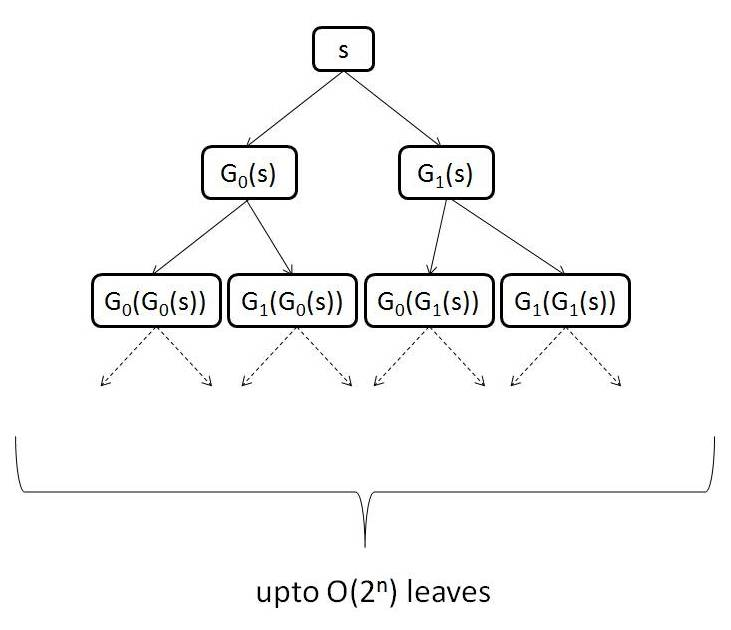
\includegraphics[width=.6\linewidth]{PRF.jpg}
  \end{center}

  Formally, we define the function $f_{s}(\cdot)$ as
  \[f_{s}(x) = G_{x_{n}}(\cdots G_{x_{2}}(G_{x_{1}}(s)) \cdots). \]
  Why might we expect $f_{s}$ to ``look random,'' for a uniformly
  random (secret) seed $s$?  Intuitively, $G_{0}(s)$ and $G_{1}(s)$
  ``look like'' independent uniform $n$-bit strings, and we might
  expect this pseudorandomness to propagate downward through the
  layers of the tree.  Let us try to prove this rigorously.

  \emph{Attempt 1}: Design a sequence of hybrid experiments where each
  leaf of the tree is successively replaced by its ``ideal'' form,
  i.e., with a uniform $n$-bit string.  Clearly, the $0$th hybrid
  corresponds to the ``real'' tree construction, and the $2^{n}$th
  corresponds to a truly random function.  However, this approach is
  flawed, as it requires $2^n$ hybrid steps.  (As an exercise, show
  that the hybrid lemma is \emph{false}, in general, for an
  exponential number of hybrid steps.)

  \emph{Attempt 2:} Successively replace each \emph{layer} of the tree
  with ideal uniform, independent entries (all at once).  Thus,
  $H_{0}$ corresponds to the real tree construction, and $H_{n}$
  corresponds to a truly random function.  Note that we now have only
  $n$ hybrid steps.

  More formally, we describe hybrid distributions defining (a
  distribution over functions) $f$ as follows:
  \begin{itemize}
  \item $H_{0}$ is the real tree construction, with a uniformly random
    root $s$, and $f(x) = G_{x_{n}}(\cdots G_{x_{1}}(s) \cdots)$.
  \item For $i \in [n]$, $H_{i}$ is the tree construction, but using
    uniformly random seeds across the $i$th layer of the tree.
    Formally, $f(x) = G_{x_{n}}(\cdots G_{x_{i+1}}(s_{x_{i}\cdots
      x_{1}})$, where the seeds $s_{y}$ are uniformly random and
    independent for each $y \in \bit^{i}$.
  \end{itemize}
  
  As a warm-up, we first show that $H_{0} \compind H_{1}$ (in the
  sense of oracle indistinguishability) assuming that $G$ is a PRG.
  To prove this, we need to construct a simulator $\Sim$ that emulates
  one of $H_{0}$ or $H_{1}$ (as oracles), depending on whether its
  input is $G(U_{n})$ or $U_{2n}$.  That is, the simulator should use
  its input to answer arbitrary queries.  The simulator $\Sim$ works
  as follows: given $(z_{0}, z_{1}) \in \bit^{2n}$, it answers each
  query $x$ by returning $G_{x_{n}}(\cdots G_{x_{2}}(z_{x_{1}})\cdots
  )$.

  It is easy to check that the simulator emulates the desired hybrids.
  First, if $(z_{0}, z_{1}) = (G_{0}(s), G_{1}(s))$ for $s \gets
  U_{n}$, then $\Sim(z_{0}, z_{1})$ answers each query $x \in
  \bit^{n}$ as
  \[ G_{x_{n}}(\cdots G_{x_{2}}(G_{x_{1}}(s)) \cdots ) = f_{s}(x), \]
  exactly as in $H_{0}$.  Similarly, if $(z_0, z_1) \gets (U_n,
  U_n)$, then $\Sim$ answers each query exactly as in $H_{1}$.  Now
  because $G(U_{n}) \compind U_{2n}$ and $\Sim$ is efficient, by the
  hybrid lemma we conclude that $H_0 \compind H_1$.

  Unfortunately, this approach does not seem to scale too well when we
  go down to the deeper layers of the tree, because the simulator
  $\Sim$ would need to take as input an exponential number of input
  strings.  However, we can make two observations:
  \begin{itemize}
  \item In $H_{i}$, all the subtrees growing from the $i$th level are
    \emph{symmetric}, i.e., they are identically distributed and
    independent.
  \item The polynomial-time distinguisher $\Dist$ attacking the PRF
    can make only a \emph{polynomial} number of queries to its oracle.
  \end{itemize}
  The key point is that the simulator then only needs to simulate
  $q(n) = \poly(n)$ number of subtrees in order to answer all the
  queries of the distinguisher correctly.

  For the hybrids $H_{i-1}$ and $H_{i}$, Algorithm~\ref{alg:simulator}
  defines a simulator that takes $q(n) = \poly(n)$ pairs of $n$-bit
  strings.
  
  \renewcommand{\algorithmicrequire}{\textbf{Input:}}

  \begin{algorithm}
    \label{alg:simulator}
    \caption{Simulator $\Sim_{i}$ for emulating either $H_{i-1}$ or $H_{i}$.}
    \begin{algorithmic}[1]
      \REQUIRE $(z^1_0, z^1_1), \ldots , (z^q_0, z^q_1) \in \bit^{2n}$
      for some large enough $q(n) = \poly(n)$
      \STATE $j \gets 1$
      \WHILE{there is a query $x \in \bit^{n}$ to answer}
      \IF{prefix $x_{1} \cdots x_{i}$ is not yet associated with any $k$}
      \STATE associate $j$ to $x_{1} \cdots x_{i}$
      \STATE $j \gets j+1$
      \ENDIF
      \STATE look up the $k$ associated with prefix $x_{1} \cdots
      x_{i}$
      \STATE answer $G_{x_{n}}(\cdots G_{x_{i+1}}(z^{k}_{x_{i}})
      \cdots)$
      \ENDWHILE
    \end{algorithmic}
  \end{algorithm}

  We analyze the behavior of $\Sim_{i}$.  Suppose that the
  distinguisher $\Dist$ (making queries to $\Sim_{i}$) makes at most
  $q$ queries, so the counter $j$ never ``overflows.''  Now, if each
  of the pairs $(z^{j}_{0}, z^{j}_{1}) \gets G(U^{j}_{n})$ are
  independent pseudorandom strings, then $\Sim_{i}$ answers each query
  $x$ by $G_{x_{n}}(\cdots (G_{x_{i+1}}(G_{x_{i}}(U^{k}_{n}))\cdots)$,
  for a distinct $k$ associated uniquely with the $i$-bit prefix of
  $x$.  By construction, $\Sim_{i}$ therefore emulates $H_{i-1}$
  exactly.  Similarly, if the $(z^{j}_{0}, z^{j}_{1}) \gets U^j_{2n}$
  are uniformly random and independent, then $\Sim_{i}$ simulates
  $H_{i}$.

  At this point, we would like to conclude that $H_{i-1} \compind
  H_{i}$, but can we?  To do so using the hybrid lemma, we would need
  to show that the two types of inputs to $\Sim_{i}$ (namely, a
  sequence of $q = \poly(n)$ \emph{independent pairs} $(z_{0}, z_{1})$
  each drawn from either $G(U_{n})$ or $U_{2n}$) are
  indistinguishable.  This can be shown via a straightforward hybrid
  argument, using the hypothesis that $G$ is a PRG, and is left as an
  exercise.
\end{proof}

\subsection{Consequences for (Un)Learnability}
\label{sec:cons-learning}

A family of functions is said to be \emph{learnable} if any member of
the family can be reconstructed efficiently (i.e., as code), given
oracle access to the function.  In this sense, a PRF family is
\emph{completely unlearnable}, in that no efficient adversary can
determine \emph{anything} about the values of the function (given
oracle access) on any of the unqueried points.  As a consequence, if a
class of functions is expressive enough to ``contain'' a PRF family,
then this class is unlearnable.  E.g., under standard assumptions, the
class $\class{NC}^{1}$ can implement PRFs, hence it is unlearnable.

\end{document}

%%% Local Variables: 
%%% mode: latex
%%% TeX-master: t
%%% End: 
